


\chapter{Experimental Evaluation of the Minimalist Prover\label{ch:proverEvaluation}}
%-----------------------------------------------------------------------------
The evaluation of the minimalist prover orbits three fundamental questions: first, does it succeed in proving verification conditions arising programs; second, are our heuristics effective at increasing the usefulness of the prover; and third, does the data gathered by the prover expose any interesting properties of VCs that arise from well-engineered programs.

The first and second questions are explored by considering a series of verification benchmarks.  In Section \ref{canProve} we present each benchmark and explore the effectiveness of the automated prover when applied to that benchmark.  Following that, in Section \ref{heuristicsEval}, we use those same benchmarks to explore how our various heuristics impact the effectiveness of the prover.  Finally, the third question is addressed in Section \ref{proverEvalConclusion}, where we provide some observations and conclusions based on the collected data.

This chapter focuses on the specifications and realizations of the benchmarks.  We defer the discussion of relevant mathematics to Chapter \ref{ch:mathEvaluation}.  We present only enough of each specification and realization to motivate our discussion, but the full specifications of each benchmark and any associated data abstractions can be found in Appendix \ref{apx:specs} and full realizations in Appendix \ref{apx:real}.  Full listings of the proofs generated as solutions to the benchmarks in this chapter are available in Appendix \ref{apx:proofs}.

While the usability of our prover and its application in educational settings is not a core part of this thesis, we take this opportunity to note that our minimalistic prover provides the backbone of the RESOLVE verifying compiler and has facilitated teaching reasoning at Clemson and a variety of other institutions.  We point the interested reader to \cite{cook2012specification} or \cite{sitaraman2009engaging} for results of experimentation with the prover in educational settings.


%-----------------------------------------------------------------------------
\section{Description of Metrics}
%-----------------------------------------------------------------------------
For this chapter we focus on four primary metrics for exploring the effectiveness of the prover and analyzing the difficulty of VCs.  These are:

\begin{itemize}
	\item \textbf{VCs proved.}  The number of VCs that are successfully dispatched by the prover.  Since the proof space is quite large, the prover often runs with a set timeout, so in reality this metric refers to the number of VCs that were proved within the timeout.  In the experiments discussed throughout this chapter, the timeout was set at 20 seconds.
	\item \textbf{Real time.}  The amount of time required to dispatch the VC, generally measured in milliseconds.  Because this metric can vary depending on a number of variables, we present the mean of of five repeated trials along with the standard deviation.
	\item \textbf{Proof steps.}  The number of relevant steps taken by the prover.  One of the features of the prover is to prune steps that do not impact the final result.
	\item \textbf{Search steps.}  A subset of the overall proof steps including only those steps taken during the ``consequent exploration'' phase described in Section \ref{consequentExploration}, and not including those consequent steps that are ``obvious'', namely: replacing a consequent that matches a given with \texttt{true}, replacing a consequent that is a symmetric equality with \texttt{true}, and eliminating a conjunct that is \texttt{true}.  Intuitively this metric refers to the number of steps that were blind exploration of the proof space and which may have to be backtracked over, rather than deterministic steps over which we do not backtrack.
\end{itemize}


%-----------------------------------------------------------------------------
\section{Benchmark Solutions\label{canProve}}
%-----------------------------------------------------------------------------

%-----------------------------------------------------------------------------
	\subsection{VSTTE Benchmarks}
%-----------------------------------------------------------------------------
In 2010, members of the RSRG at Clemson and The Ohio State University published a set of incremental verification benchmarks at the Verified Software: Tools, Theories, and Experiments conference (VSSTE)\cite{Benchmarks}.  These benchmarks are intended to provide a basis for experimentation and discussion among verification efforts.  In \cite{hartonDissertation}, the author presents a selection of these benchmarks implemented in RESOLVE in order to demonstrate the VC-generation capabilities of the RESOLVE compiler.  We mirror that methodology in this section, presenting a selection of the VSTTE benchmarks, including several that are borrowed or adapted from \cite{hartonDissertation}, before applying our minimalist prover to them and presenting resulting data.
	%-----------------------------------------------------------------------------
		\subsubsection{Benchmark 1: Adding and Multiplying Integers}
	%-----------------------------------------------------------------------------

\paragraph{Problem Statement}Verify an operation that adds two numbers by repeated incrementing. Verify an operation that multiplies two numbers by repeated addition, using the first operation to do the addition. Make one algorithm iterative, the other recursive.\footnote{This and all other problem statements quote directly from \cite{Benchmarks}.}

\paragraph{Solution Discussion}In Listing \ref{lst:integerAddMultSpec} we present specifications of integer addition and multiplication operations in RESOLVE.  Each of these operations is specified to work ``in place'', transforming the first parameter (which is also used as one of the inputs) into the final solution.

\lstinputlisting[float=h,language=resolve,caption={The specification of \texttt{Adding\_Capabilitiy} and \texttt{Multiplying\_Capability}\label{lst:integerAddMultSpec}}]{proverEval/examples/IntegerPlusTimesSpecs.en}

Each operation specifies that its second parameter must be positive---dealing correctly with the presence of negative numbers adds a surprising amount of implementation complexity for a language like RESOLVE that strives to correctly reason about bounded integers, since the maximum and minimum integer are generally not symmetrical.  Note, however, that we lose no generality---a more general addition or multiplication function could be specified and wrapped around the ones presented in this section, transforming any addition or multiplication task into a finite subset of tasks that could computed correctly by these implementations.

We experimented both with an iterative and recursive implementation of \texttt{Adding\_Capability}.  We present the rescursive implementation in Listing \ref{lst:addImpl}.  Note that the \texttt{decreasing} clause currently lists the integer \texttt{j}, but once we have a true theory of ordinals we would like for such clauses to take an ordinal.  The iterative implementation of \texttt{Adding\_Capability} is available in Appendix \ref{apx:specs}.

\lstinputlisting[float=h,language=resolve,caption={A recursive implementation of \texttt{Adding\_Capability}\label{lst:addImpl}}]{proverEval/examples/Recursive_Add_to_Realiz.rb}

Our implementation of \texttt{Multiplying\_Capabilitiy} is iterative and presented in Listing \ref{lst:multImpl}.

\lstinputlisting[float=h,language=resolve,caption={An iterative implementation of \texttt{Multiplying\_Capability}\label{lst:multImpl}}]{proverEval/examples/Iterative_Multiply_into_Realiz.rb}

\begin{sloppypar}
Integer syntax is built-in to RESOLVE for convenience, though Integers are specified and used through concepts like any other data abstraction. This makes using one enhancement to \texttt{Integer\_Template} from another fairly unweildy, which is why we do not use \texttt{Adding\_Capability} to implement \texttt{Multiplying\_Capability} as requested by the benchmark, but rather the normal integer \texttt{+}. We note, however, that \texttt{+} is drawn from \texttt{Integer\_Template} as a normal specification and thus presents the same verification challenges (that is: reasoning about it is not built in).
\end{sloppypar}

\paragraph{Results}Each of the three implementations is fully verifiable.  The results of those verifications, with associated metrics are presented in Figure \ref{fig:addMultResults}.

\begin{figure}
	\centering
	\begin{subfigure}[b]{0.45\textwidth}
		\centering
		\begin{tabular}{lrrrr}
			\toprule
				& Time (ms)	& $\sigma$& Steps & Search \\
			\midrule
			VC 0\_1	& 5560		& 182	& 5	& 0     \\
			VC 0\_2	& 3456		& 280	& 5	& 0     \\
			VC 0\_3	& 565		& 78	& 10	& 0     \\
			VC 0\_4	& 834		& 197	& 9	& 0     \\
			VC 0\_5	& 3873		& 219	& 6	& 0     \\
			VC 0\_6	& 613		& 101	& 8	& 0     \\
			VC 0\_7	& 591		& 106	& 5	& 0     \\
			VC 1\_1	& 5020		& 286	& 9	& 0     \\
			\bottomrule
		\end{tabular}
		\caption{Iterative \texttt{Adding\_Capabilitiy} results\label{fig:iterAddResults}}
	\end{subfigure}
	\qquad
	\begin{subfigure}[b]{0.45\textwidth}
		\centering
		\begin{tabular}{lrrrr}
			\toprule
				& Time (ms)	& $\sigma$& Steps & Search \\
			\midrule
			VC 0\_1	& 2549		& 124	& 9	& 0     \\
			VC 0\_2	& 1244		& 221	& 9	& 0     \\
			VC 0\_3	& 977		& 177	& 5	& 0     \\
			VC 0\_4	& 1379		& 222	& 6	& 0     \\
			VC 0\_5	& 1118		& 159	& 6	& 0     \\
			VC 0\_6	& 757		& 82	& 8	& 0     \\
			VC 0\_7	& 1113		& 178	& 5	& 0     \\
			VC 1\_1	& 379		& 76	& 8	& 0     \\
			\bottomrule
		\end{tabular}
		\caption{Recursive \texttt{Adding\_Capabilitiy} results\label{fig:recAddResults}}
	\end{subfigure}

	\vspace{2em}
	\begin{subfigure}[b]{0.6\textwidth}
		\centering
		\begin{tabular}{lrrrr}
			\toprule
				& Time (ms)	& $\sigma$& Steps & Search \\
			\midrule
			VC 0\_1	& 6264		& 195	& 7	& 0     \\
			VC 0\_2	& 3484		& 365	& 5	& 0     \\
			VC 0\_3	& 3495		& 182	& 7	& 2     \\
			VC 0\_4	& 393		& 149	& 7	& 0     \\
			VC 0\_5	& 333		& 53	& 5	& 0     \\
			VC 1\_1	& 5917		& 124	& 8	& 0     \\
			\bottomrule
		\end{tabular}
		\caption{Iterative \texttt{Multiplying\_Capabilitiy} results\label{fig:iterMultResults}}
	\end{subfigure}
  \caption{Results from verification of Benchmark 1 solutions\label{fig:addMultResults}}
\end{figure}

\FloatBarrier
%-----------------------------------------------------------------------------
		\subsubsection{Benchmark 2: Binary Search an Array}
%-----------------------------------------------------------------------------

\paragraph{Problem Statement}Verify an operation that uses binary search to find a given entry in an array of entries that are in sorted order.

\paragraph{Solution Discussion}In Listing \ref{lst:searchSpec} we present a specification of a searching operation on an array.  The operation takes as its input an entry and an array in sorted order, then uses a parameterizable comparison function, \texttt{LEQ}, to search the array.

\lstinputlisting[float=h,language=resolve,caption={The specification of \texttt{Searching\_Capabilitiy}\label{lst:searchSpec}}]{proverEval/examples/Search_Capability.en}

The \emph{requires} clause of the operation uses higher-order definitions to establish that the array is in order---i.e., that it is \emph{conformal} with the given comparator.  The \emph{ensures} clause states that the operation will return \texttt{true} if and only if the given entry exists between the lower and upper bound of the array.  The details of these higher-order definitions are explored more fully in Chapter \ref{ch:mathEvaluation}.

An implementation for this operation is provided in Listing \ref{lst:searchImpl}.

\lstinputlisting[float=t,language=resolve,caption={An implementation of \texttt{Searching\_Capabilitiy}\label{lst:searchImpl}}]{proverEval/examples/Bin_Search_Realiz.rb}

The realization takes a function, \texttt{Are\_Ordered()} which provides a programmatic way of establishing \texttt{LEQ}.  From there, the implementation is the usual straightforward binary search implementation.  Note that when calculating the new mid, we first take the difference, then divide, avoiding the overflow problem exposed in \cite{blochBinarySearch}.

An important design goal of RESOLVE is that as much reasoning as possible happens through the general component machinery.  As a result, RESOLVE does not elevate arrays (or pointers, as we discuss in \cite{kulczyckiPointers}) to special status, unlike nearly all other practical verification languages (\cite{DafnyOverview}, \cite{cok:esc}, or \cite{kuncakJahobOverview}, e.g.).

\FloatBarrier

While we provide syntactic sugar for array operations, they are supported by an ordinary component that provides specifications for all array operations, a snippet of which is provided in Listing \ref{lst:arraySpec}.

\lstinputlisting[float=!h,language=resolve,caption={A snippet of the specification of arrays\label{lst:arraySpec}}]{proverEval/examples/Static_Array_Template.co}

\paragraph{Results} Of the 45 VCs generated by this example, we are able to mechanically verify 39.  These results are summarized in Figure \ref{fig:binSearchResults}.

\begin{figure}[t]
	\centering
	\begin{tabular}{lrrrr}
		\toprule
			& Time (ms)	& $\sigma$& Steps & Search \\
		\midrule
		VC 0\_1	& 1411		& 174 	& 6 	& 1     \\
		VC 0\_2	& 819		& 161	& 5 	& 0     \\
		VC 0\_3	& 573		& 107	& 5 	& 0     \\
		VC 1\_1	& 2523		& 249	& 8 	& 0     \\
		VC 1\_2	& 1607		& 148	& 5	& 0     \\
		VC 1\_3	& 1318		& 111	& 5 	& 0     \\
		VC 1\_4	& 792		& 155	& 5 	& 0     \\
		VC 1\_5	& 6438		& 261	& 10	& 3     \\
		VC 1\_6	& 2401		& 302	& 9 	& 1     \\
		VC 1\_7	& 6838 		& 178	& 10	& 3     \\
		VC 1\_8	& 2430 		& 188	& 9	& 1     \\
		VC 1\_9	& \multicolumn{4}{c}{Not Proved}        \\
		VC 1\_10 & 2108		& 191	& 7 	& 1     \\
		VC 1\_11 & 2097		& 305	& 5 	& 0     \\
		VC 1\_12 & \multicolumn{4}{c}{Not Proved}       \\
		VC 1\_13 & 3259		& 309	& 9	& 3     \\
		VC 2\_1	& 1637		& 116	& 8 	& 0     \\
		VC 2\_2	& 1346		& 98	& 5	& 0     \\
		VC 2\_3	& 1361		& 99	& 5 	& 0     \\
		VC 2\_4	& 595		& 35	& 5 	& 0     \\
		VC 2\_5	& 5816		& 247	& 10	& 3     \\
		VC 2\_6	& 2414		& 121	& 9 	& 1     \\
		VC 2\_7	& 6465 		& 338	& 10	& 3     \\
		\bottomrule
	\end{tabular}
	\quad
	\begin{tabular}{lrrrr}
		\toprule
			& Time (ms)	& $\sigma$& Steps & Search \\
		\midrule
		VC 2\_8	& 2813 		& 187	& 9	& 1     \\
		VC 2\_9	& \multicolumn{4}{c}{Not Proved}        \\
		VC 2\_10 & 2923		& 393	& 11	& 4     \\
		VC 2\_11 & 2369		& 260	& 5 	& 0     \\
		VC 2\_12 & \multicolumn{4}{c}{Not Proved}       \\
		VC 2\_13 & 11229	& 204	& 8	& 3     \\
		VC 3\_1	& 1715		& 124	& 8 	& 0     \\
		VC 3\_2	& 1322		& 139	& 5	& 0     \\
		VC 3\_3	& 1242		& 140	& 5 	& 0     \\
		VC 3\_4	& 630		& 64	& 5 	& 0     \\
		VC 3\_5	& 6095		& 151	& 10	& 3     \\
		VC 3\_6	& 2540		& 306	& 9	& 1     \\
		VC 3\_7	& 6388 		& 335	& 10	& 3     \\
		VC 3\_8	& 2730 		& 230	& 9	& 1     \\
		VC 3\_9	& \multicolumn{4}{c}{Not Proved}        \\
		VC 3\_10 & 2386		& 228	& 5 	& 0     \\
		VC 3\_11 & 2785		& 300	& 10	& 2     \\
		VC 3\_12 & \multicolumn{4}{c}{Not Proved}       \\
		VC 3\_13 & 18032	& 273	& 9	& 2     \\
		VC 4\_1	& 2474		& 70	& 9 	& 3     \\
		VC 4\_2	& 787		& 129	& 5	& 0     \\
		VC 4\_3	& 813		& 71	& 5 	& 0     \\
		\bottomrule
	\end{tabular}
	\caption{Binary search \texttt{Searching\_Capabilitiy} results\label{fig:binSearchResults}}
\end{figure}

The six VCs that are not mechanically verified represent a failure not of the prover---but rather of RESOLVE's underlying syntax.  Because at this time RESOLVE does not permit the application of an arbitrary expression (as opposed to a named function), we are unable to formulate the required theorems to prove these VCs.

We now present a manual proof of a representative one of these VCs by hand and argue that once this syntactic problem is resolved, our minimalist prover will be easily able to dispatch the VC.

Consider the VC in Listing \ref{lst:brokenVC} corresponding to the inductive case of the while loop's maintaining clause.  Irrelevant givens have been omitted for brevity.

\lstinputlisting[float=!h,language=resolve,caption={A problematic VC\label{lst:brokenVC}}]{proverEval/examples/BrokenVC.asrt}

Let us now proceed as the mechanical prover would.  We first replace instances of \texttt{A''} with \texttt{A}, resulting in the givens shown in Listing \ref{lst:givens2}.

\begin{lstlisting}[float=!h,language=,caption={New givens after replacing \texttt{A''} with \texttt{A}\label{lst:givens2}}]
A' = lambda ( j : Z ).(
	{{midVal'' if j = (low'  + ((high'  - low')  / 2))
	  A(j) otherwise}}) and
A((low'  + ((high'  - low')  / 2))) = key)
\end{lstlisting}

We now replace \texttt{A'} with its full expansion in the goal, resulting in the new goal shown in Listing \ref{lst:goal2}.

\begin{lstlisting}[float=!h,language=,caption={New goal after expanding \texttt{A'}\label{lst:goal2}}]
lambda ( j : Z ).(
	{{key if j = (low'  + ((high'  - low')  / 2))
	  lambda ( j : Z ).(
		{{midVal'' if j = (low'  + ((high'  - low')  / 2))
	  	A(j) otherwise}}(j) otherwise}})
= A
\end{lstlisting}

Finally, we replace instances of \texttt{key} with its expansion, resulting in the final goal shown in Listing \ref{lst:goal3} (we change the internal lambda's variable to \texttt{k} for clarity, though the prover does not have to deal with this complication).

\begin{lstlisting}[float=!h,language=,caption={New goal after expanding \texttt{key}\label{lst:goal3}}]
lambda ( j : Z ).(
	{{A((low'  + ((high'  - low')  / 2))) 
		if j = (low'  + ((high'  - low')  / 2))
	  lambda ( k : Z ).(
		{{midVal'' if k = (low'  + ((high'  - low')  / 2))
	  	A(k) otherwise}})(j) otherwise}})
= A
\end{lstlisting}

At this point we are able to apply the theorem given in Listing \ref{lst:lambdaThm} (note that it applies a function-valued expression when it evaluates a lambda expression at \texttt{x} and therefore cannot be represented in our current syntax).

\begin{lstlisting}[float=!h,language=resolve,caption={A useful theorem about lambda expressions\label{lst:lambdaThm}}]
Theorem Shadowed_Function_Piece:
	For all T, R : MType,
	For all t : T,
	For all r : R,
	For all f : T -> R,
		f = lambda (x : T).(
			{{f(x) if x = t;
			  lambda (y : Z).(
				{{r if y = t;
				  f(y) otherwise}})(x) otherwise}});
\end{lstlisting}

We are then left with simply \texttt{A~=~A}, at which point the remainder of the proof is trivial.  Each of these six VCs has a similar straightforward proof.

\FloatBarrier
%-----------------------------------------------------------------------------
		\subsubsection{Benchmark 3: Sorting a Queue}	
%-----------------------------------------------------------------------------

\paragraph{Problem Statement}Specify a user-defined FIFO queue ADT that is generic (i.e., parameterized by the type of entries in a queue). Verify an operation that uses this component to sort the entries in a queue into some client-defined order.

\paragraph{Solution Discussion}In Listing \ref{lst:sortingSpec} we present a specification of a queue sorting enhancement.  As with Benchmark 2, it takes as a parameter a client-provided definition to define the sorted order, \texttt{LEQV}.  It uses two higher-order definitions \texttt{Is\_Coformal\_With()} and \texttt{Is\_Permutation()} to ensure that the final queue is ordered according to \texttt{LEQV} and contains the same elements as those original provided, respectively.

\lstinputlisting[float=h,language=resolve,caption={The specification of \texttt{Sorting\_Capability}\label{lst:sortingSpec}}]{proverEval/examples/Sorting_Capability.en}

A straightforward selection sort realization is provided in Listing \ref{lst:sortingImpl}.

\lstinputlisting[float=!h,language=resolve,caption={A selection sort realization of \texttt{Sorting\_Capabilitiy}\label{lst:sortingImpl}}]{proverEval/examples/Selection_Sort_Realization.rb}

Again, as in Benchmark 2, we take a client-provided operation, \texttt{Compare()}, that implements \texttt{LEQV}, and use it to implement our \texttt{Remove\_Min()} sub-operation.  The \texttt{One()} and \texttt{Two()} procedures simply provide a way of getting the programmatic values \texttt{1} and \texttt{2} using a normal specification.

\paragraph{Results}This implementation is fully verifiable.  The results of that verifications, with associated metrics, is presented in Figure \ref{fig:sortingResults}.  Based on our literature review, we believe that RESOLVE is the only verification effort with a generic, automatically-verifiable selection sort\footnote{The RESOLVE group at The Ohio State University has their own version of this automatically-verifiable selection sort.  We note, however, that their system takes advantage of a specialized decision procedure for reasoning about strings, whereas our solution uses only our generalized minimalist prover.}.  One notable automatically-verifiable attempt is from a series of implementations of the VSTTE benchmarks in Dafny\cite{DafnySolutions}, but that solution operates only on integers where ours is generic.

\begin{figure}[!h]
	\centering
	\begin{tabular}{lrrrr}
		\toprule
			& Time (ms)	& $\sigma$& Steps & Search \\
		\midrule
		VC 0\_1	& 1344		& 242 	& 6 	& 0     \\
		VC 0\_2	& 479		& 73	& 5 	& 0     \\
		VC 0\_3	& 912		& 56	& 5 	& 0     \\
		VC 0\_4	& 1305		& 198	& 6 	& 1     \\
		VC 0\_5	& 2762		& 300	& 8	& 0     \\
		VC 0\_6	& 3128		& 372	& 9 	& 3     \\
		VC 0\_7	& 1513		& 271	& 8 	& 0     \\
		VC 0\_8	& 1710		& 136	& 10	& 1     \\
		VC 0\_9	& 2219		& 166	& 9 	& 3     \\
		VC 1\_1	& 501 		& 100	& 5 	& 0     \\
		VC 1\_2	& 1012 		& 165	& 10	& 1     \\
		VC 2\_1	& 806 		& 136	& 5 	& 0     \\
		VC 2\_2	& 1918		& 237	& 8 	& 0     \\
		VC 2\_3	& 1781		& 197	& 5 	& 0     \\
		VC 2\_4	& 1620		& 284	& 6 	& 1     \\
		VC 2\_5	& 3021		& 387	& 14	& 0     \\
		\bottomrule
	\end{tabular}
	\qquad
	\begin{tabular}{lrrrr}
		\toprule
			& Time (ms)	& $\sigma$& Steps & Search \\
		\midrule
		VC 2\_6	& 4441		& 278	& 12	& 3     \\
		VC 2\_7	& 1919		& 108	& 10	& 2     \\
		VC 2\_8	& 1843		& 139	& 7 	& 0     \\
		VC 3\_1	& 819 		& 141	& 5 	& 0     \\
		VC 3\_2	& 1896		& 213	& 8 	& 0     \\
		VC 3\_3	& 1642		& 124	& 5 	& 0     \\
		VC 3\_4	& 1493		& 197	& 6 	& 1     \\
		VC 3\_5	& 2965		& 239	& 14	& 0     \\
		VC 3\_6	& 4202		& 200	& 10	& 1     \\
		VC 3\_7	& 1897		& 194	& 10	& 2     \\
		VC 3\_8	& 1863		& 165	& 7 	& 0     \\
		VC 4\_1	& 838 		& 139	& 5 	& 0     \\
		VC 4\_2	& 2939		& 150	& 12	& 0     \\
		VC 4\_3	& 1132		& 189	& 5 	& 0     \\
		VC 4\_4	& 3056		& 262	& 18	& 3     \\
		\bottomrule
	\end{tabular}
	\caption{Selection sort \texttt{Sorting\_Capabilitiy} results\label{fig:sortingResults}}
\end{figure}

\FloatBarrier
%-----------------------------------------------------------------------------
	\subsection{Other Benchmarks}
%-----------------------------------------------------------------------------

%-----------------------------------------------------------------------------
		\subsubsection{Reversing a Queue\label{sec:reversingAQueue}}	
%-----------------------------------------------------------------------------

\paragraph{Problem Statement}Specify a user-defined FIFO queue ADT that is generic (i.e., parameterized by the type of entries in a queue). Verify an operation that reverses the entries in a given queue.

\paragraph{Solution Discussion}In Listing \ref{lst:flippingSpec} we present a specification of a queue reversing enhancement called \texttt{Flipping\_Capability}.  A recursive solution follows in Listing \ref{lst:flippingImpl}.


\lstinputlisting[float=h,language=resolve,caption={The specification of \texttt{Flipping\_Capabilitiy}\label{lst:flippingSpec}}]{proverEval/examples/Flipping_Capability.en}

\lstinputlisting[float=h,language=resolve,caption={A recursive realization of \texttt{Flipping\_Capabilitiy}\label{lst:flippingImpl}}]{proverEval/examples/Recursive_Flipping_Realiz.rb}

\paragraph{Results}This implementation is fully verifiable.  The results of that verifications, with associated metrics, is presented in Figure \ref{fig:flippingResults}.

\begin{figure}
	\centering
	\begin{tabular}{lrrrr}
		\toprule
			& Time (ms)	& $\sigma$& Steps & Search \\
		\midrule
		VC 0\_1	& 1520		& 141	& 5 	& 0     \\
		VC 0\_2	& 3118		& 295	& 7 	& 0     \\
		VC 0\_3	& 2741		& 222	& 8 	& 0     \\
		VC 0\_4	& 2174		& 170	& 9 	& 2     \\
		VC 1\_1	& 366		& 83	& 10	& 0     \\
		\bottomrule
	\end{tabular}
	\caption{Recursive \texttt{Flipping\_Capabilitiy} results\label{fig:flippingResults}}
\end{figure}

\paragraph{Implicit vs. Explicit Style}As formulated here, \texttt{Queue\_Template} uses an \emph{implicit} style for specifying the \texttt{Dequeue()} operation.  We reproduce that specification in Listing~\ref{lst:implicitDequeue} for convenience.

\begin{lstlisting}[float=h,language=resolve,caption={An implicit-style specification for \texttt{Dequeue()}\label{lst:implicitDequeue}}]
Operation Dequeue(replaces R: Entry; updates Q: Queue);
	requires |Q| /= 0;
	ensures #Q = <R> o Q;
\end{lstlisting}

In implicit style, the final values of one or more parameters are described via properties they will have, rather than by a mapping to an explicit value.  Here, both the final value of \texttt{Q} and of \texttt{R} will be such that combining them will yield the original value of the queue, \texttt{\#Q}.  The alternative is \emph{explicit} style, in which \texttt{Q} and \texttt{R} would be explicitly mapped to a final value.  An example of this style is given in Listing~\ref{lst:explicitDequeue}.

\begin{lstlisting}[float=h,language=resolve,caption={An explicit-style specification for \texttt{Dequeue()}\label{lst:explicitDequeue}}]
Operation Dequeue(replaces R: Entry; updates Q: Queue);
	requires |Q| /= 0;
	ensures R = Element_At(0, #Q) and Q = Substring(#Q, 1, |#Q| - 1);
\end{lstlisting}

One interesting question is whether the choice of style of specification has an impact on the verifiability of the flip operation.  Verifying \texttt{Flip()} again, this time using the explicit style specification, provides the results shown in Figure~\ref{fig:explicitFlippingResults}.  Note that because this example does not involve a separate realization, we do not include these results in the aggregate results in Section~\ref{heuristicsEval} or Section~\ref{proverEvalConclusion}.

\begin{figure}
	\centering
	\begin{tabular}{lrrrr}
		\toprule
			& Time (ms)	& $\sigma$& Steps & Search \\
		\midrule
		VC 0\_1	& 2199		& 160	& 5 	& 0     \\
		VC 0\_2	& 1468		& 182	& 6 	& 0     \\
		VC 0\_3	& 2149		& 253	& 8 	& 0     \\
		VC 0\_4	& 1589		& 225	& 8 	& 3     \\
		VC 1\_1	& 845		& 139	& 10	& 0     \\
		\bottomrule
	\end{tabular}
	\caption{Recursive \texttt{Flipping\_Capabilitiy} results, based on an explicitly-specified queue\label{fig:explicitFlippingResults}}
\end{figure}

Total, using an explicit specification required 1669 milliseconds longer than implicit style.  It saved two proof steps overall, but cost an additional search step.  Taken together, none of this data suggests one style or the other as clearly better.

%-----------------------------------------------------------------------------
		\subsubsection{Array Realization of Stack}	
%-----------------------------------------------------------------------------

\paragraph{Problem Statement}Specify a user-defined LIFO stack ADT that is generic (i.e., parameterized by the type of entries in a queue). Verify an array implementation of that ADT.

\paragraph{Solution Discussion}Listing \ref{lst:stackSpec} gives RESOLVE's specification for a stack in the context of a \texttt{Stack\_Template}, which is generic and bounded.

\lstinputlisting[float=h,language=resolve,caption={The specification of \texttt{Stack}\label{lst:stackSpec}}]{proverEval/examples/Stack_Template.co}

We implement this specification on top of an array, which, as in Benchmark 2, is a first-class component with its own template and operation specifications.  This array-based implementation is provided in Listing \ref{lst:stackImpl}.

\lstinputlisting[float=h,language=resolve,caption={An array-based implementation of \texttt{Stack}\label{lst:stackImpl}}]{proverEval/examples/Array_Realiz.rb}

\paragraph{Results}This implementation is fully verifiable.  The results of that verifications, with associated metrics, is presented in Figure \ref{fig:stackResults}.

\begin{figure}
	\centering
	\begin{tabular}{lrrrr}
		\toprule
			& Time (ms)	& $\sigma$& Steps & Search \\
		\midrule
		VC 0\_1	& 493		& 58	& 5 	& 0     \\
		VC 1\_1	& 4116		& 552	& 7 	& 0     \\
		VC 2\_1	& 240		& 132	& 5 	& 0     \\
		VC 2\_2	& 4324		& 268	& 7 	& 1     \\
		VC 2\_3	& 200		& 42	& 6 	& 0     \\
		VC 3\_1	& 18583		& 490	& 7 	& 2     \\
		VC 3\_2	& 2331		& 516	& 8 	& 0     \\
		VC 3\_3	& 1709		& 178	& 6 	& 1     \\
		VC 3\_4	& 2038		& 83	& 8 	& 0     \\
		VC 3\_5	& 2243		& 475	& 9 	& 2     \\
		VC 4\_1	& 6592 		& 314	& 11	& 3     \\
		VC 4\_2	& 1187		& 234	& 5 	& 0     \\
		VC 4\_3	& 891		& 216	& 9 	& 0     \\
		VC 4\_4	& 1124		& 142	& 6 	& 1     \\
		\bottomrule
	\end{tabular}
	\qquad
	\begin{tabular}{lrrrr}
		\toprule
			& Time (ms)	& $\sigma$& Steps & Search \\
		\midrule
		VC 4\_5	& 956		& 291	& 7 	& 0     \\
		VC 5\_1	& 1558 		& 408	& 5 	& 0     \\
		VC 5\_2	& 2070		& 300	& 5 	& 0     \\
		VC 5\_3	& 1705		& 299	& 7 	& 0     \\
		VC 5\_4	& 1769		& 428	& 5 	& 0     \\
		VC 6\_1	& 1668 		& 465	& 5 	& 0     \\
		VC 6\_2	& 2344		& 300	& 5 	& 0     \\
		VC 6\_3	& 2217		& 386	& 7 	& 0     \\
		VC 6\_4	& 1729		& 392	& 5 	& 0     \\
		VC 7\_1	& 625 		& 146	& 5 	& 0     \\
		VC 7\_2	& 1390		& 342	& 7 	& 0     \\
		VC 7\_3	& 598		& 169	& 4 	& 0     \\
		VC 7\_4	& 683		& 217	& 6 	& 0     \\
		\bottomrule
	\end{tabular}
	\caption{Array-based \texttt{Stack} implementation results\label{fig:stackResults}}
\end{figure}

\FloatBarrier
%-----------------------------------------------------------------------------
		\subsubsection{Do Nothing on Trees}	
%-----------------------------------------------------------------------------
\paragraph{Problem Statement}Specify a tree abstraction, then specify, implement, and verify an operation that modifies the a tree before restoring it to its original form.

\paragraph{Solution Discussion}Clearly, the usefulness of this benchmark is not in the operation itself, which is trivial.  Rather, this benchmark is designed to demonstrate the flexibility of our mathematical system by allowing us to showcase a proof-of-concept implementation involving trees and reasoning about using that implementation the same machinery as any other construct.

Listing \ref{lst:treeSpec} gives a small snippet of a RESOLVE specification for a generic n-ary tree in the context of a \texttt{Tree\_Template}.

\lstinputlisting[float=h,language=resolve,caption={A specification of \texttt{Tree}\label{lst:treeSpec}}]{proverEval/examples/Tree_Template.co}

The function \texttt{Get\_Root()} returns the value at the root of the tree, while \texttt{Split()} returns each of the child subtrees of the specified tree as a \texttt{Str(Tree(Entity))}.  The mathematical basis for trees is discussed in more detail in Chapter \ref{ch:mathEvaluation}.

We then specify an operation on trees, \texttt{Do\_Nothing()}, shown in \ref{lst:doNothingSpec}.  Note that the requires clause is in place simply to allow us to make some initial modification to the tree before restoring it to its original form.

\lstinputlisting[float=h,language=resolve,caption={A \texttt{Do\_Nothing()} operation on \texttt{Tree}\label{lst:doNothingSpec}}]{proverEval/examples/Do_Nothing_Capability.en}

Finally, we implement this operation in a straightforward way in Listing \ref{lst:doNothingImpl}.  First we add an arbitrary subtree, then we remove it again.

\lstinputlisting[float=h,language=resolve,caption={A straightforward implementation of \texttt{Do\_Nothing}\label{lst:doNothingImpl}}]{proverEval/examples/Obvious_Do_Nothing_Realiz.rb}

\paragraph{Results}This implementation is fully verifiable.  The results of that verifications, with associated metrics, is presented in Figure \ref{fig:treeResults}.

\begin{figure}[h]
	\centering
	\begin{tabular}{lrrrr}
		\toprule
			& Time (ms)	& $\sigma$& Steps & Search \\
		\midrule
		VC 0\_1	& 2899		& 129	& 5 	& 0     \\
		VC 0\_2	& 1782		& 241	& 6 	& 1     \\
		VC 0\_3	& 3471		& 372	& 11 	& 0     \\
		\bottomrule
	\end{tabular}
	\caption{Simple \texttt{Do\_Nothing\_Capabilitiy} results\label{fig:treeResults}}
\end{figure}

%-----------------------------------------------------------------------------
\section{Heuristic Evaluation\label{heuristicsEval}}
%-----------------------------------------------------------------------------
In order to evaluate the effectiveness of our heuristics from Section \ref{domainSpecific}, the prover has been instrumented so that each of six different heuristics could be disabled individually.  The heuristics we targetted are: ignoring useless transformations, developing the antecedent only about relevant terms, focusing on diversity in antecedent development, minimizing both consequent and antecedent, cycle detection, and transformation prioritization.

We then re-ran the verification process on each of the benchmarks and collected data about the changes to our various metrics.  This data is summarized in Figure \ref{heuristicEvalTable}.  Time here is based on the median of three repeated trials, simply to eliminate outlier times.

\setlength{\tabcolsep}{7pt}
\begin{figure}
	\centering
	\begin{tabular}{lrrrrrrr}
		\toprule
			& $\sum \Delta\text{\footnotesize Proved}$	& $\overline{\Delta t / \sigma}$	& $\sum\Delta t$ & $\overline{\Delta\text{\footnotesize steps}}$ & $\sum\Delta\text{\footnotesize steps}$ & $\overline{\Delta\text{\footnotesize search}}$ & $\sum\Delta\text{\footnotesize search}$ \\
		\midrule
		\footnotesize With useless \\
		\footnotesize transformations		& -12	& 4.07	& 83438		& 0	& 0	& 0	& 0	\\
		\midrule
		\footnotesize Developing about \\
		\footnotesize irrelevant terms		& -1	& 8.80	& 154530	& 0	& 0	& 0	& 0\\
		\midrule
		\footnotesize Not checking for \\
		\footnotesize diversity of givens	& -6	& -5.55	& -142026	& -0.02	& -4	& -0.01	& -1	\\
		\midrule
		\footnotesize No minimization		& -10	& 2.53	& 36651		& 0.02	& 3	& 0.28	& 35	\\
		\midrule
		\footnotesize No cycle detection	& 0	& 0.60	& 9629		& 0.08	& 11	& 0.08	& 11	\\
		\midrule
		\footnotesize No prioritization \\
		\footnotesize of transformations	& -19	& 2.60	& 17577		& 0.05	& 6	& 0.04	& 5	\\
		\bottomrule
	\end{tabular}
	\caption{Summary of heuristic evaluation results.  From left to right the columns are: total change in the number of proved VCs (negative means fewer were proved), average standard deviations change in time to prove, total change in time to prove, average change to the number of steps required, total change in number of steps required, average change in number of search steps required, and total change in number of search steps required.  Average and total changes only take into account VCs that were proved.\label{heuristicEvalTable}}
\end{figure}
\setlength{\tabcolsep}{6pt}

As expected, we see that the heuristics are at least partially responsible for a number of VCs being proved.  Ignoring useless transformations, limiting development to relevant terms, diversifying antecedents, minimizing, and prioritizing transformations all make the difference between some VCs proving or not proving.  Of those, it is interesting to note that diversifying antecedents poses a trade off---it requires more time (2 minutes, 37 seconds on these 133 VCs), but it enabled six more VCs to prove.  This may indicate that it would benefit from being targetted for further optimization to reduce the cost of applying it.  On the other hand, ignoring useless transformations, limiting development to relevant terms, minimization, and prioritization are nothing but a net gain.  They are collectively responsible for speeding up the proving process by over four and a half minutes and permitting 43 additional VCs to prove (though, for both time and the provability of VCs we imagine that there is an overlap in the time saved and VCs proved and thus this is not a strictly additive relationship).

An important metric is the change in search steps, since from an algorithmic perspective these steps are the most expensive to take: they contribute to the overall combinatorial explosion of time as we must inductively search deeper and deeper for a solution.  We note that three of our heuristics improve this metric, while only one has adverse effects (and a small one at that).  All told, we may summarize the net effect of all our heuristics as saving 51 search steps.

It may at first be unclear how minimization can eliminate thirty-five search steps but only three total proof steps---after all, search steps are a subset of total proof steps.  Consider, however, that minimization is a heuristic for taking \emph{extra steps} that are likely to be useful.  The discrepancy of thirty-two steps represent steps that were \emph{not} taken in the preprocessing phase, but instead delayed to the consequent exploration phase.  This increases the complexity of the search as steps taken in the exporation phase contribute to the combinatorial explosion of the search space, while steps taken in the preprocessing phase do not.


%-----------------------------------------------------------------------------
\section{Observations and Conclusions\label{proverEvalConclusion}}
%-----------------------------------------------------------------------------
These six examples were chosen to be representative of the sorts of problems to which our prover can be applied, but do not constitute the total body of components we can automatically verify.  We have a library of many other verified operations operating on stacks, queues, lists, and integers.

These benchmarks together involve 133 VCs ranging over the mathematical domains of functions, trees, strings, integers, and booleans.  Of those, we are able to mechanically verify 127, with the remaining 6 provable module improvements to RESOLVE's language representation.  This is visualized in Figure \ref{fig:pie}.  Of the mechanically verifiable VCs, the median time to prove was 1809 milliseconds, and the mean time was 2493 milliseconds.  The median number of proof steps was seven and the median number of search steps was zero.

\begin{figure}
	\centering
	\begin{subfigure}[b]{0.40\textwidth}
		\centering
		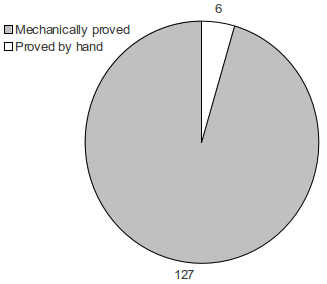
\includegraphics[width=\textwidth]{proverEval/proofResults3.png}
		\caption{Verification results\label{fig:pie}}
	\end{subfigure}
	\quad
	\begin{subfigure}[b]{0.55\textwidth}
		\centering
		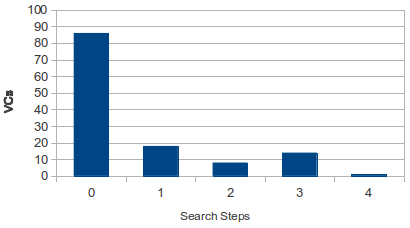
\includegraphics[width=\textwidth]{proverEval/searchSteps2.png}
		\caption{Number of Search Steps Required by Proofs\label{fig:histogram}}
	\end{subfigure}
	\caption{Summary of Proof Evaluation Results}
\end{figure}

As we have previously mentioned, we are particularly interested in the search step metric since it represents the only non-deterministic portion of the proof search.  That the median number of such steps is zero is extremely heartening and we are further encouraged that no VC required more than four.  Figure \ref{fig:histogram} shows a histogram of the number of VCs requiring different numbers of search steps.

The majority (86, or 65\%) of VCs required no search steps once all heuristics were applied.  40 (30\%) required three or fewer steps, while only a single VC required four search steps.  This data supports our hypothesis that VCs arising from well-engineered software should require only simple analysis with a minimalist prover to dispatch.
